\section{Additional technologies used in selection}
\label{ref:sel:tech}

All technologies described in this selection has been employed in the previous
analysis (\cite{LHCb-ANA-2020-056}), which uses LHCb run 1 data, but has been
updated to work with LHCb run 2 data.
Only a brief description for each technology is reproduced here.
For more details, refer to \cite{LHCb-ANA-2014-052,LHCb-ANA-2020-056}.

\subsection{Isolation BDT}
\label{ref:sel:tech:iso-bdt}

A multivariate BDT, referred as ``isolation BDT'',
conceptually identical to the one used in \cite{LHCb-ANA-2020-056},
is trained on LHCb run 2 simulation
%with training variables listed in \cref{tab:iso-bdt-input},
to provide a score-based estimation on if a charged track is originating from
the \B ($D^{(*)}\mu$) vertex or not.

The isolation BDT is applied on all charged tracks in the event,
providing isolation scores for each of them where
higher score implies higher probability of coming from the \B vertex, named as
``anti-isolated''.
Three tracks with highest isolation scores\footnote{
    The ones that are most likely to be anti-isolated.
} are saved in descending order\footnote{
    So the first one is the most anti-isolated one among all charged tracks
    in the event.
}.


\subsection{Veto of overlapping candidates}
\label{ref:sel:tech:veto}

% See this note: https://github.com/umd-lhcb/rdx-run2-analysis/blob/master/docs/cuts/Dst_veto_in_D0.md
Since the selection of a \Dstar\muon pair always requires the existence
of a \Dz\muon pair,
there is about 21\% of events in the signal (ISO) skim of the \Dstar channel
leaks into \Dz channel.
% 21 computed as: 630178 (overlap) / 3011082 (num of evt for D0)
%%%%
This is likely due to the fact that slow \pion typically has poor tracking
resolution (small \ipChiSq), making the slow \pion to be more likely
\emph{unassociated} with the \Dz\mun vertex thus the reconstruction of \Dstar
would fail.

To veto the overlapping candidates between \Dz and \Dstar channel,
a tool, named \smalltt{TupleToolApplyIsolationVetoDst},
is added to the selection procedure, which processes all tracks
in the event in the following manner:

\begin{enumerate}
    \item Denote the track as $t$.
    \item Refit a vertex from \Dz and $t$.
    \item Compute $\Delta m_\text{veto} \equiv m_{\Dz t} - m_\Dz$.
    \item Test if $\Delta m_\text{veto} \in [140~\text{GeV}, 160~\text{GeV}]$.
        If it is, the track $t$ is able to form a \Dstar-like particle with \Dz,
        and the $\Delta m_\text{veto}$ and isolation BDT score
        of the track are recorded.
\end{enumerate}

From all recorded BDT scores and $\Delta m_\text{veto}$, the
$\Delta m_\text{veto}$ of the tracks with top two BDT scores are saved
for future use.
It is then required offline (listed in \cref{tab:offline-cut-d0})
that these two tracks,
the best slow \pion candidates,
are \emph{incompatible} with
forming a \Dz\pion vertex with a mass close to \Dstar reference mass.

Note that this tool does not rank tracks based \emph{solely} on the isolation:
The poor tracking resolution of the slow \pion makes the association of
the track more ambiguous; sometime the track may be associated with the PV,
instead of the \B vertex, in which case the track would receive a small BDT
score.
By ranking based on the BDT scores of the tracks that fall within the
$[140~\text{GeV}, 160~\text{GeV}]$
$\Delta m_\text{veto}$ window only,
it is more robust to retain the best slow \pion candidates,
as reported in \cite{LHCb-ANA-2020-056}.

In addition, an alternative mass hypothesis is tested
(offline, also listed in \cref{tab:offline-cut-d0}), where the reconstructed
\muon is treated as a \pion,
and $\Delta m_\text{alt hypo} = m_{\Dz\muon_\text{as \pion}} - m_\Dz$
is computed\footnote{
    By using the 3-momentum of the \muon, while using $m_\pion$ as the invariant
    mass of the track.
} and required to be inconsistent with \Dstar PDG mass.

The veto procedures are applied on all samples of the \Dz channel only.


\subsection{Muon PID}
\label{ref:sel:tech:ubdt}

To maintain minimum bias on \muon \pt, a multivariate BDT,
referred as \UBDT, using \texttt{uBDT} method in TMVA class,
is trained to reject misidentified \muon while keeping rejection
efficiency flat on \pt,
as described in \cite{LHCb-ANA-2020-056}.

The \UBDT has been re-trained on LHCb run 2 MC samples.
There is ongoing effort to study its efficiency against standard run 2 PID
variables.
Early report suggests the flatness on \pt is maintained while rejection
efficiencies relative to existing PID cut are high for all but proton ($p$),
as shown in \cref{fig:ubdt-eff}.

% Generated with:
%   https://github.com/umd-lhcb/pidcalib2, branch efficiency_study
% first, run efficiency_gen/rdx-run2-ubdt-misidgen.sh
% then, go inside scripts folder, run ./plots.py
\begin{figure}[htb]
    \centering
    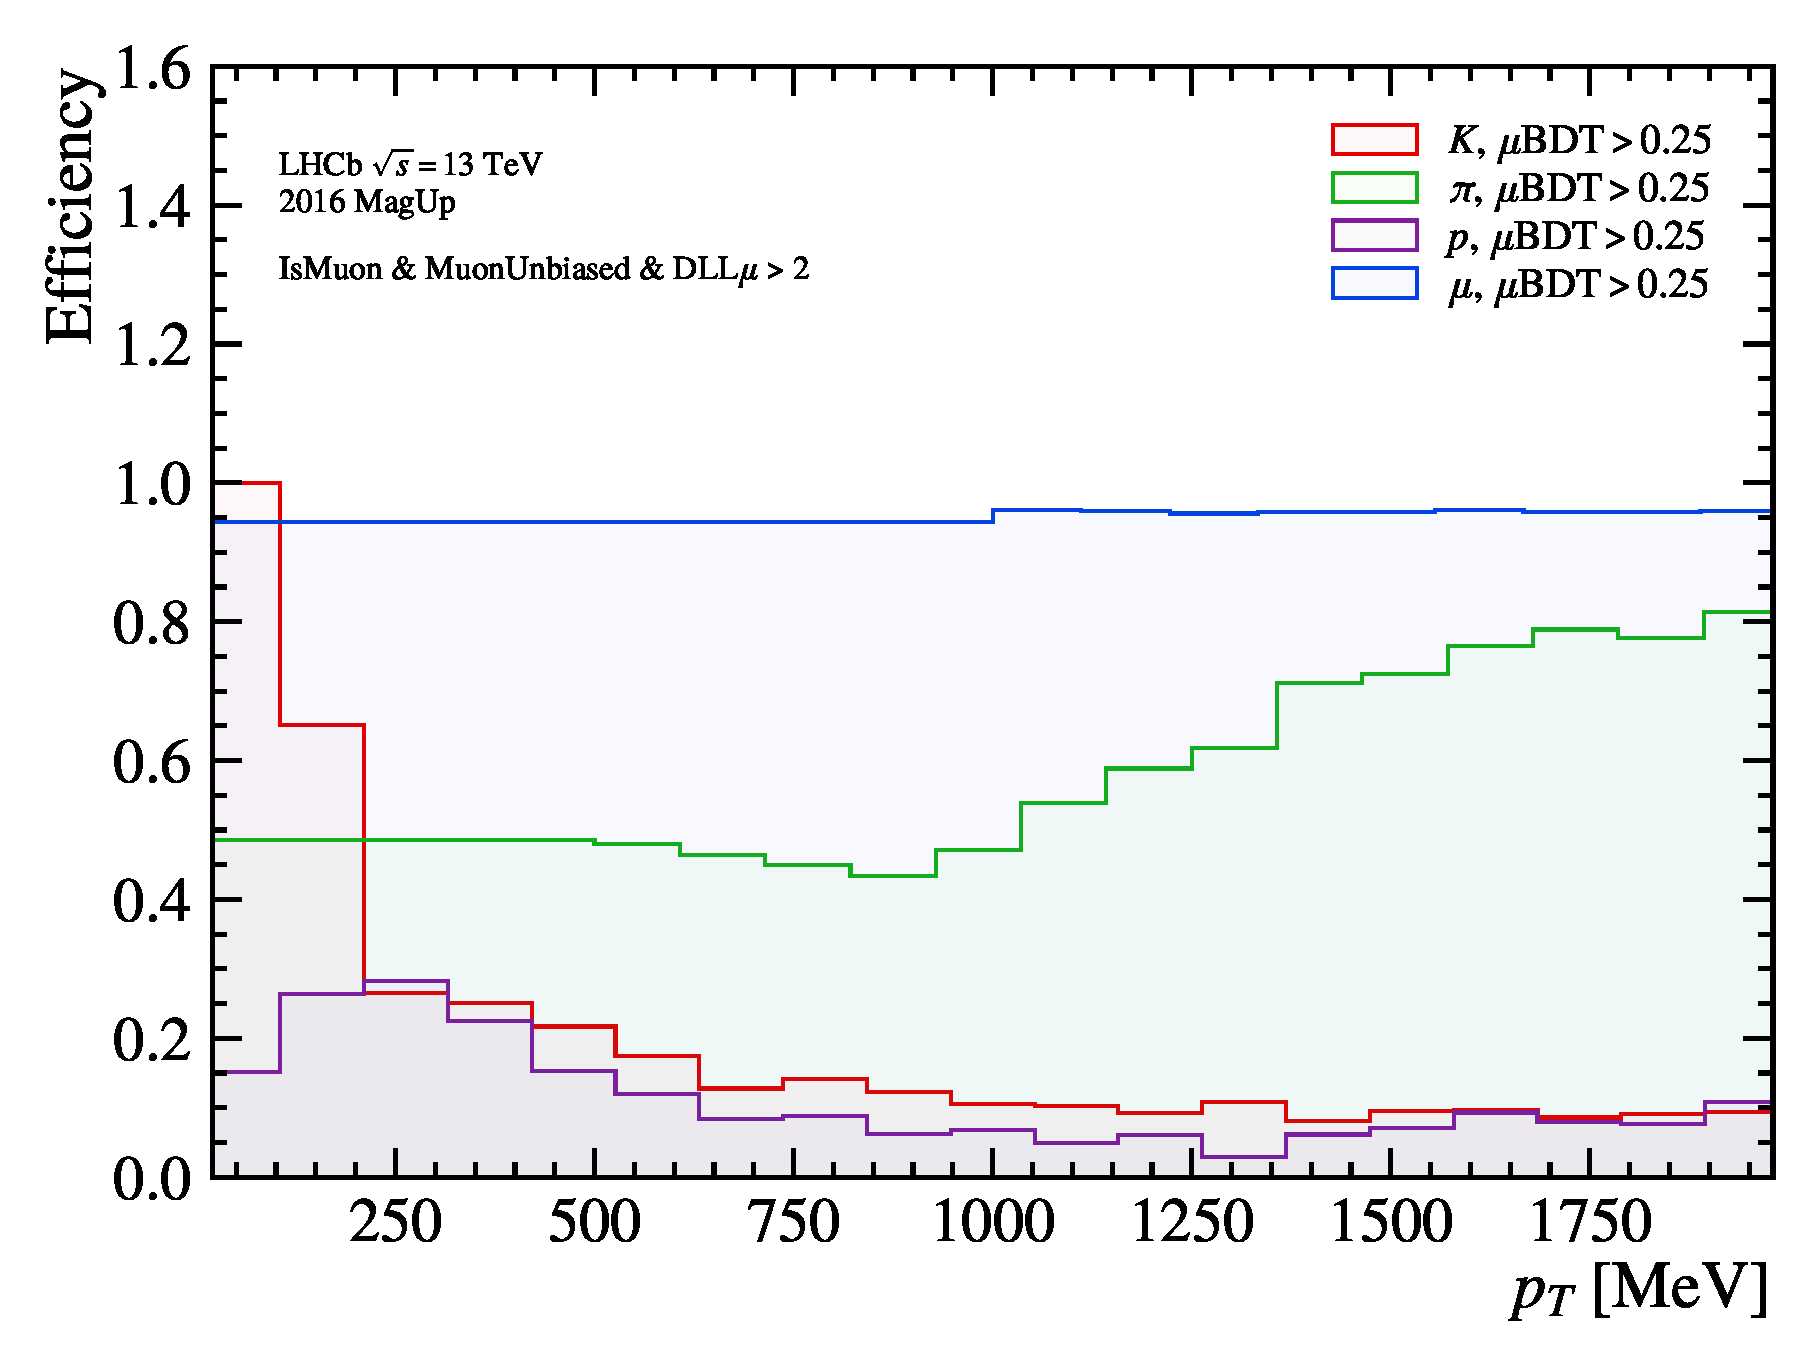
\includegraphics[width=0.45\textwidth]{./figs-selection-tech/eff_Brunel_PT_up_pidcalib_ubdt_eff.pdf}
    \hspace{1em}
    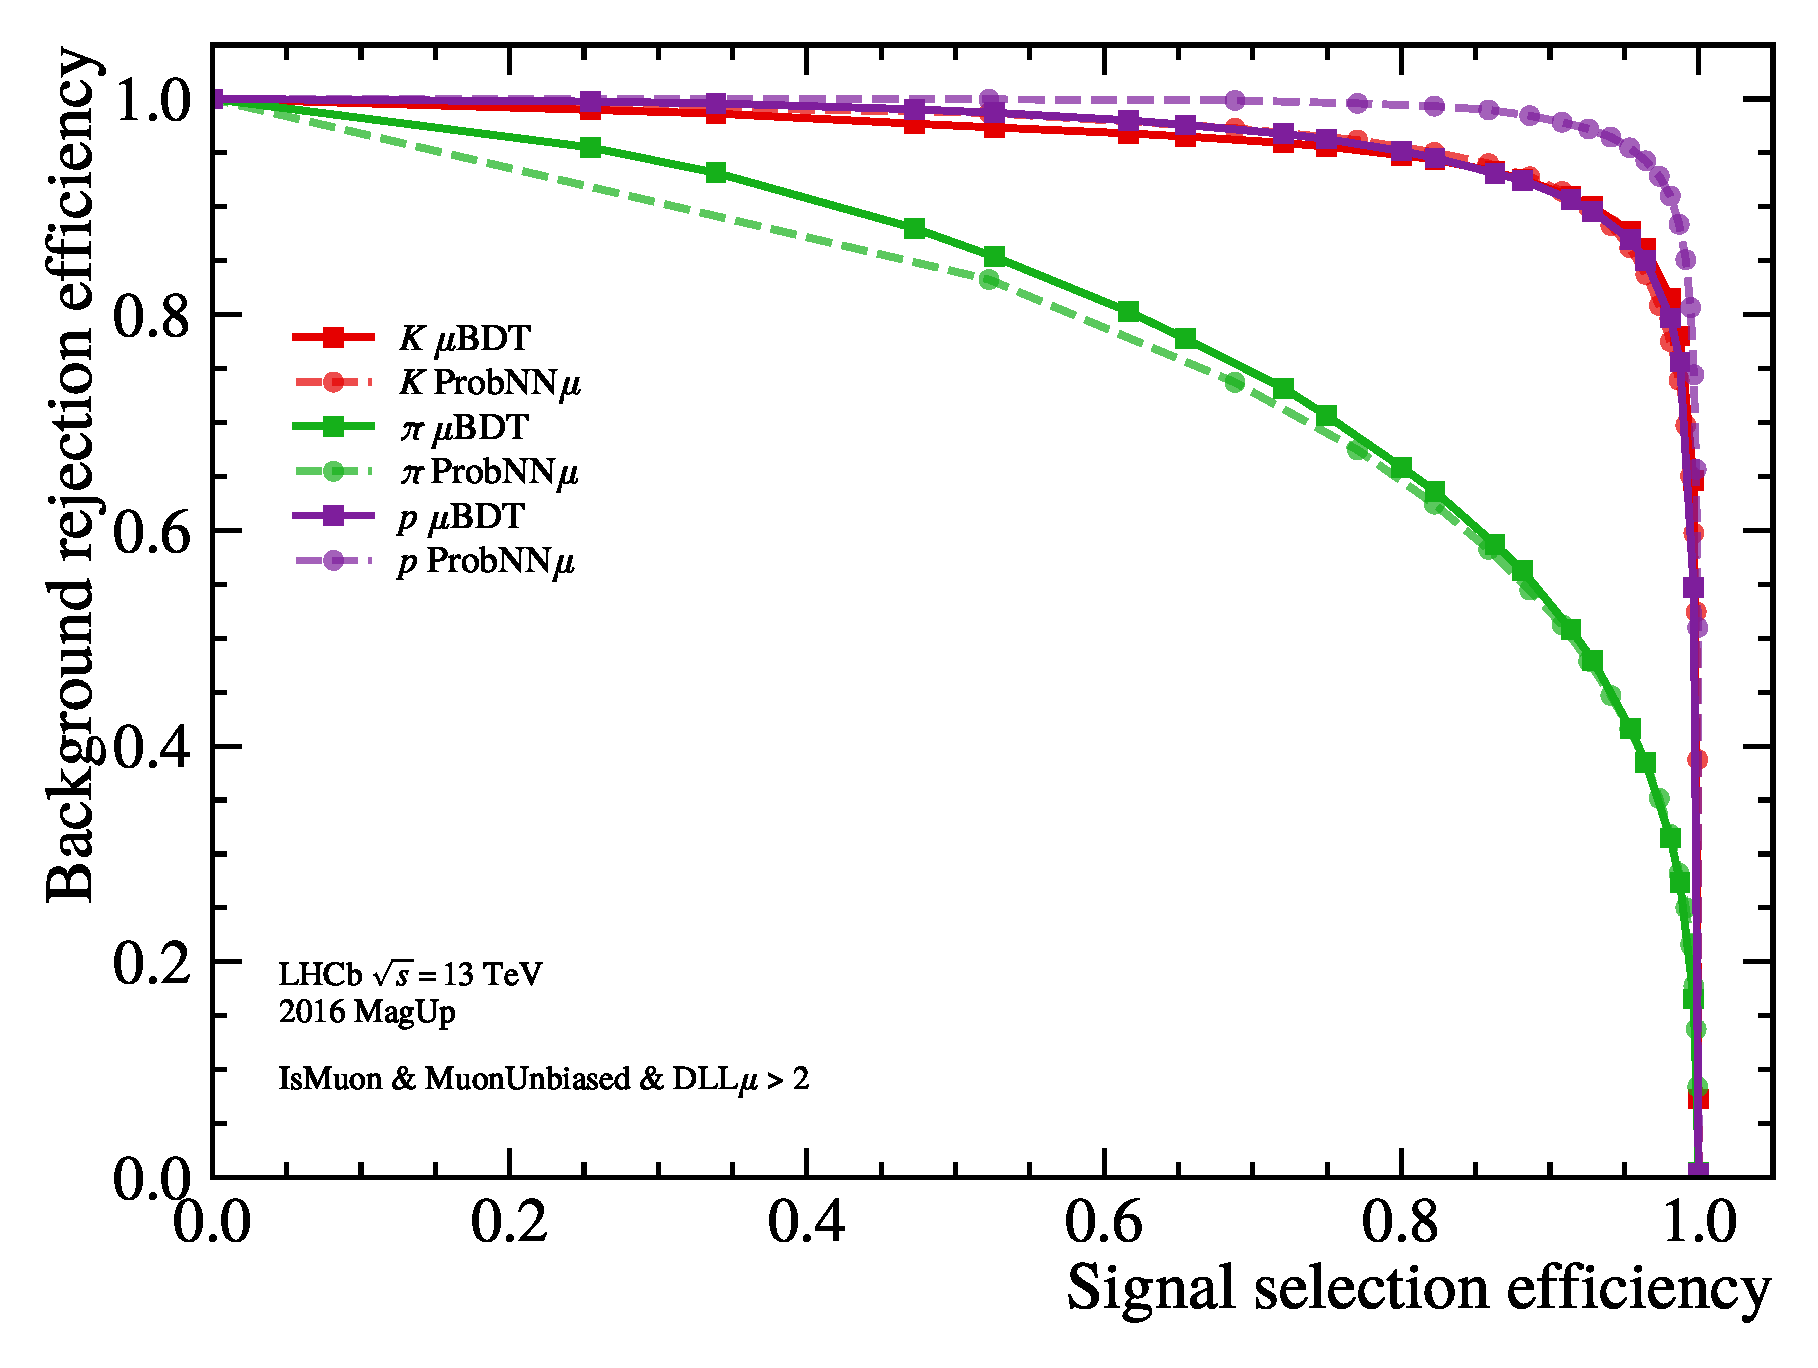
\includegraphics[width=0.45\textwidth]{./figs-selection-tech/rej_v_eff_unbiased_Brunel_PT.pdf}

    \caption{
        Preliminary \UBDT study.
        Left: \UBDT \muon selection efficiency is flat in \pt, with
        global cut \isMuon \& $\text{\PID{\muon}}\! > 2$,
        and $\UBDT > 0.25$.
        Right: with the same global cut, \UBDT is more effective in rejecting
        \pion than LHCb official \ProbNN{\muon}.
        The \kaon rejection efficiencies are similar between the two;
        the $p$ rejection efficiency is lower for \UBDT, but the absolute
        rejection efficiency is high enough.
    }
    \label{fig:ubdt-eff}
\end{figure}
